\section{Auswertung}

\textit{Hinweis: Soweit nicht anders angegeben, werden im folgenden Abschnitt alle Fehler nach der standardmäßigen Gauß'schen Fehlerfortpflanzung berechnet.}

\subsection{Betrieb als Kältemaschine und quantitative Bestimmung der Kälteleistung}

Zentral für die Bestimmung des Wirkungsgrades ist die Relation
\begin{align}
    \eta = \frac{Q_2}{W_M}
\end{align}
dabei entspricht die dem oberen Zylinderteil entzogene Wärmemenge $Q_2$ gerade der elektrischen Arbeit $W_H$, für die Kompensation durch die Heizung. Gemessen haben wir die Größen $I_H$, $U_H$ zur Bestimmung der Leistung $P_H$ der Heizung, sowie die Umlaufzahl $f$ des Schwungrades. Mit diesen gilt der Zusammenhang
\begin{align}
    Q_2 = W_M = \frac{P_H}{f} = \frac{I_H U_H}{f}.
\end{align}
Damit erhalten wir für $Q_2$ einen Wert von
\begin{align*}
    Q_2 = (4.21 \pm 0.05) \si{\joule}.
\end{align*}
Die Wärmemenge $Q_1$, welche an das Kühlwasser abgegeben wird, berechnen wir über die kalorische Zustandsgleichung
\begin{gather}
    Q_1 = \frac{c_W \rho_W \Delta T \dot{V}}{f} \label{eq:kalo_zust}\\
    \intertext{mit}
    \Delta Q_1 = Q_1 \cdot \sqrt{\relerrsq{(\Delta T)} + \relerrsq{\dot{V}} + \relerrsq{f}}.
\end{gather}
Dafür setzen wir einen Durchfluss von $\dot{V} = (4.205 \pm 0.012) \unit{\meter\squared\per\second}$ und eine Temperaturdifferenz von $\Delta T = (1.70 \pm 0.15) \si{\kelvin}$ ein. Für die Wärmekapazität von Wasser verwenden wir den im Skript angegebenen Wert von $c_w = 4180 \si{\joule\per\kilo\gram\kelvin}$, für die Dichte den Wert $\rho_W = 997\si{\kilo\gram\per\meter\cubed}$. Damit erhalten wir einen Wert von
\begin{align}
    Q_1 = (5.6 \pm 0.5) \si{\joule}.
\end{align}

Wie dem Messprotokoll zu entnehmen ist, stammen in den bisherigen Rechnungen Werte wie die Drehzahl $f$ und der Durchfluss $\dot{V}$ aus einer Reihe von $N$ Messungen $x_i$. Für diese, sowie alle folgenden Fälle verwenden wir den klassischen Mittelwert 
\begin{gather}
\overline{x} = \frac{1}{N}\sum_{i = 1}^N x_i, 
\intertext{sowie dem Standardfehler des Mittels nach}
\sigma_{\overline{x}} = \frac{1}{\sqrt{N}}\sqrt{\frac{1}{N - 1}\sum_{i = 1}^N\qty(\overline{x} - x_i)^2}
\end{gather}
und rechnen mit $x = \overline{x} \pm \sigma_{\overline{x}}$.

Zur Bestimmung der pro Umdrehung zugeführten mechanischen Arbeit durch den Motor ziehen wir die Werte $I_M$ und $U_M$ aus dem zweiten Aufgabenteil heran. Dies ist erlaubt, da der Motor für beide Versuchsteile unter den gleichen Bedingungen betrieben wurde. Mit diesen Werten gilt
\begin{align}
    W_M &= \frac{U_M I_M}{f} = (9.6 \pm 0.5) \si{\joule}.
\end{align}

Mit den nun berechneten Werten würde im idealen Fall die Energiebilanz $Q_1 = Q_2 + W_M$ gelten. Diese ist allerdings nur theoretisch erreichbar. In unserem Versuchsaufbau verzeichnen wir eine Energie von 
\begin{align}
    \Delta Q = Q_2 + W_M - Q_1 = (8.1 \pm 0.7) \si{\joule},
\end{align}
welche aus dem System verloren geht. Gründe dafür werden im Diskussionsteil näher beleuchtet werden.

Zunächst berechnen wir mit dem zu Beginn eingeführten Bruch den Wirkungsgrad der Kälteleistung zu
\begin{align}
    \eta = 0.440 \pm 0.022,
\end{align}
also in etwa $44\%$.

\subsection{Betrieb als Kältemaschine und Wärmepumpe}

Abbildung \abbref{fig:tempverlauf_kalt} zeigt dem Temperaturverlauf des Wassers im Reagenzglas, welches am oberen Zylinderbereich angebracht ist.

\begin{figure}[H]
    \centering
    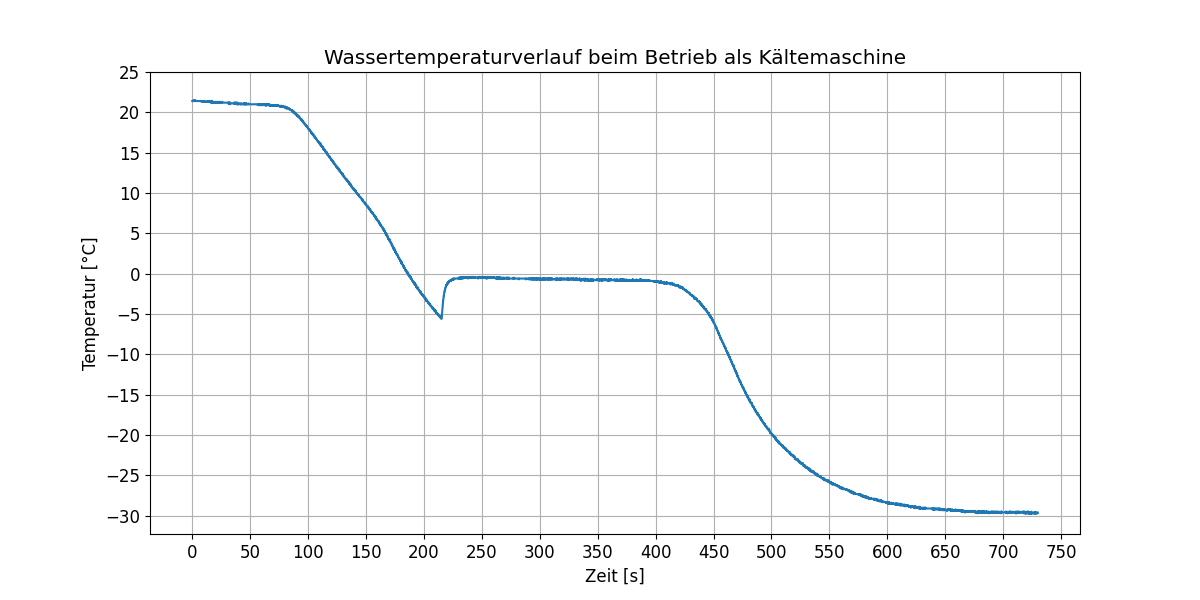
\includegraphics[width=.9\textwidth]{files/tempverlauf_kalt.png}
    \caption{Wassertemperaturverlauf beim Betrieb als Kältemaschine für etwa $1 \si{\milli\liter}$ Wasser.}
    \label{fig:tempverlauf_kalt}
\end{figure}

Der Verlauf der Temperatur zeigt, ausgehen von der Ausgangstemperatur von etwa $22\si{\celsius}$, einen nahezu perfekt linearen abfall bis zur $0\si{\celsius}$. Wir können hier einen sehr kurzen Zeitraum beobachten, in dem sich das lineare Verhalten bis $-5\si{\celsius}$ fortsetzt, um kurz darauf sehr abrupt wieder auf $0\si{\celsius}$ zu springen. Dieses Verhalten des Wassers ist auf den Effekt der \textit{Unterkühlung} zurückzuführen. Dabei wird das Wasser unter den Gefrierpunkt abgekühlt, ohne dass der Phasenübergang einsetzt. Eben dieser dann einsetzende Phasenübergang ist es, welcher für das nachfolgende Plateau von etwa 230s bis 380s verantwortlich ist. Während der Gefrierzeit, $t_f$, wird hierbei nahezu alle Energie für den Übergang des Wassers von flüssig zu fest benötigt. Erst nachdem das Wasser vollständig gefroren ist, sinkt die Temperatur weiter ab, bis sie bei ca. $-30 \si{\celsius}$ ein asymptotisches Minimum erreicht. Diese untere Grenze ist durch die maximale Kühlleistung der Kältemaschine bestimmt. 

\begin{figure}[H]
    \centering
    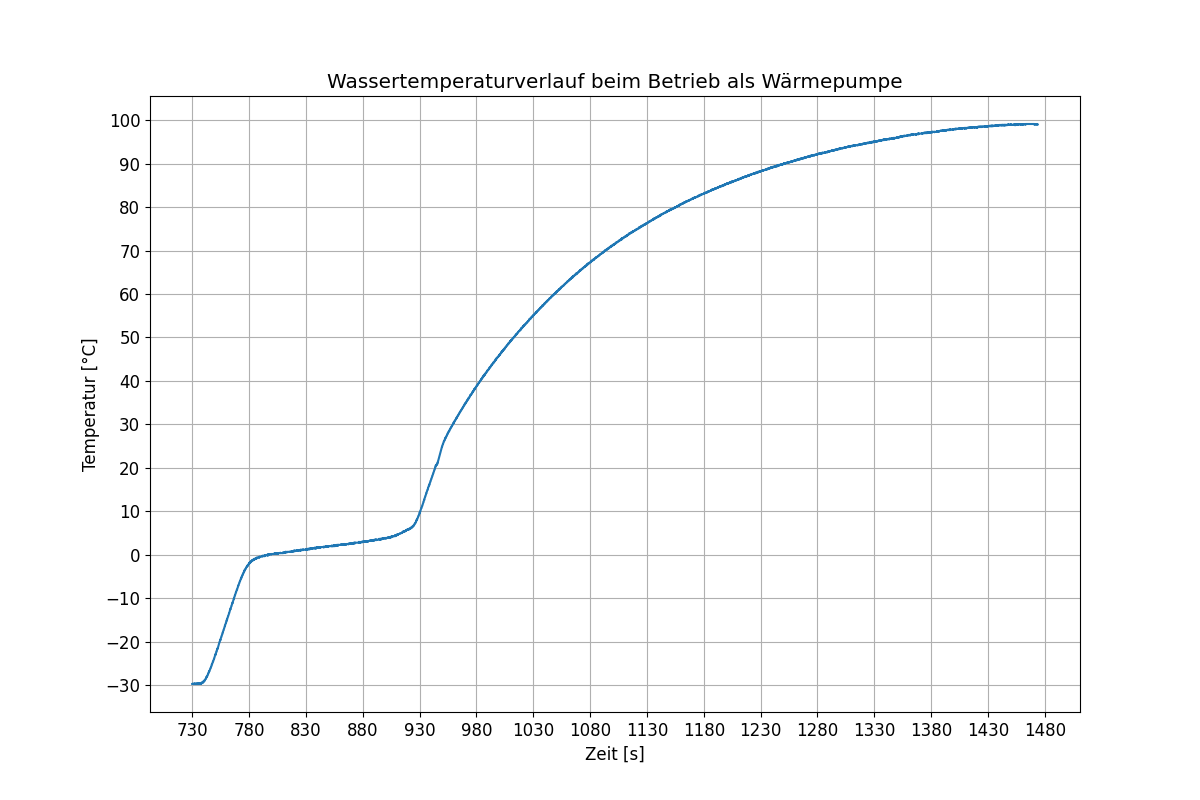
\includegraphics[width=.9\textwidth]{files/tempverlauf_warm.png}
    \caption{Wassertemperaturverlauf beim Betrieb als Wärmepumpe für etwa $1 \si{\milli\liter}$ Wasser.}
    \label{fig:tempverlauf_warm}
\end{figure}

Der Temperaturverlauf beim Betrieb als Wärmepumpe, zu sehen in \abbref{fig:tempverlauf_warm}, zeigt im Wesentlichen das gleiche Verhalten, nur in umgekehrter Reihenfolge. Was allerdings besonders auffällt, ist, dass der gesamte Prozess der Erwärmung des Wassers wesentlich schneller abzulaufen scheint. Dies könnte unter anderem durch einen Beitrag der Umgebungswärme, eine gezieltere Wärmeübertragung, und einen weniger energieintensiven Phasenübergang verursacht sein.

Nun möchten wir zusätzlich in diesem Versuchsteil die Kälteleistung der Kältemaschine berechnen. Dazu verwendeten wir die Gefrierzeit $t_f = (180 \pm 2)\si{\second}$, welche wir aus der Länge des Plateaus im Temperaturverlauf bestimmt haben. Für die notwendige Energie, um die Menge $V_W$ Wasser zu vollständig zu gefrieren gilt der Zusammenhang
\begin{align}
    \Delta E_G = V_W \rho_W \lambda_W = m_W \lambda_W.
\end{align}
Dabei ist $\lambda_W = 335\si{\joule\per\gram}$ die spezifische Schmelzwärme von Wasser. Die Kälteleistung erhalten wir daraus nach
\begin{align}
    P_G = \frac{\Delta E_G}{t_f}.
\end{align}
Diese entspricht schließlich nach unseren Messungen einem Wert von
\begin{align}
    P_G &= (1.856 \pm 0.021)\si{\joule\per\second}.
\end{align}

\subsection{Betrieb als Wärmekraftmaschine}

Wir installieren am oberen Zylinderteil nun erneut die Heizwendel, um den Motor als Wärmekraftmaschine zu betreiben. Die Heizwendel führt die elektrische Energie $Q_{el}$ in Form von Wärme zu, welche der Motor zum Teil in die mechanische Arbeit $W_{mech}$ umwandelt. Die zugeführte Energie teilt sich allerdings noch weiter auf, die komplette Energiebilanz lautet hierbei
\begin{align}
    Q_{el} = Q_v + W_{mech} + Q_{ab} + Q_R
\end{align}
$Q_v$ beschreibt Verluste bedingt durch Wärmeabstrahlung und Wärmeleitung, zusammen mit den Reibungsverlusten $Q_R$ fassen wir diese Verluste zusammen zu
\begin{align}
    Q_{V} = Q_v + Q_R.
\end{align}
Gemeinsam mit der Wärme $Q_{ab}$, welche ungenutzt ins Kühlsystem abgeführt wird, können wir die Gleichung
\begin{align}
    Q_{V} = Q_{el} - Q_{ab} - W_{mech} \label{eq:Q_V}
\end{align}
zur Berechnung der Verluste aufstellen.

$Q_{el}$ bestimmen wir anhand der Heizleistung pro Motorzyklus nach
\begin{align}
    Q_{el} = \frac{P_{el}}{f} = \frac{I_H U_H}{f}.
\end{align}
Die abgeführte Wärme $Q_{ab}$ lässt sich erneut anhand der kalorischen Zustandsgleichung \eqref{eq:kalo_zust} bestimmen. $P_{ab}$ entspricht gerade dem Zusammenhang $P_{ab} = Q_{ab} f$.

Die mechanische Arbeit $W_{mech}$ bestimmen wir nach zwei verschiedenen Methoden. Erstere macht sich die Fläche der $pV$-Diagramme zunutze. Die $pV$-Diagramme hatten wir während dem Versuch mit der Software \textit{Cassy-Lab} aufgezeichnet. Diese erlaubt uns außerdem, direkt ein Integral über die Fläche des aufgezeichneten Diagramms zu berechnen. Diese entspricht der Arbeit $W_{pV} (= Q_{pV})$, welche wir lediglich zur Vergleichbarkeit in Joule umrechnen. Auch hier ist $P_{pV}$ durch $Q_{pV}\cdot f$ gegeben.

Eine andere Variante, um die mechanische Arbeit zu berechnen nutzt das Drehmoment durch den Bremszaum aus. Dieser war von der Antriebswelle aus über einen Hebel der Länge $l$ mit einem Federkraftmesser verbunden. Aus der eingestellten Kraft können wir das ausgeübte Drehmoment bestimmen nach
\begin{align}
    D = l F.
\end{align}
Für die Arbeit abgegebene pro Motorzyklus $W_D$ gilt dann der einfache Zusammenhang
\begin{align}
    W_D = 2 \pi D = \frac{P_D}{f}.
\end{align}

Wir berechnen die angegebenen Werte zunächst für die Leerlaufmessung ohne, dass der Bremszaum angebracht ist, diese sind \tabref{tab:werte_leerlauf} zu entnehmen. 

\begin{table}[h!]
    \centering
    \begin{tabular}{l | c | c | c | c | c | c | c | c}
    \textbf{} & \boldmath$f\,\qty[\si{\per\second}]$ & \boldmath$P_{\text{el}}\,\qty[\si{\joule\per\second}]$ & \boldmath$Q_{\text{el}}\,\qty[\si{\joule}]$ & \boldmath$P_{\text{ab}}\,\qty[\si{\joule\per\second}]$ & \boldmath$Q_{\text{ab}}\,\qty[\si{\joule}]$ & \boldmath$P_{pV}\,\qty[\si{\joule\per\second}]$ & \boldmath$Q_{pV}\,\qty[\si{\joule}]$ & \boldmath$\eta_{\text{th}}$ \\\hline
    Wert & $4.815$ & $144.8$ & $30.08$ & $57.3$ & $11.9$ & $7.49$ & $1.556$ & $0.0517$ \\\hline
    Fehler & $\pm 0.011$ & $\pm 0.7$ & $\pm 0.16$ & $\pm 2.5$ & $\pm 0.6$ & $\pm 0.09$ & $\pm 0.017$ & $\pm 0.0007$ \\
    \end{tabular}
    \caption{Berechnete Werte aus der Leerlaufmessung}
    \label{tab:werte_leerlauf}
\end{table}

Der hier aufgeführte thermische Wirkungsgrad $\eta_{th}$ entspricht dem Verhältnis der mechanischen Arbeit zur zugeführten Wärme
\begin{align}
    \eta_{th} = \frac{W_{pV}}{Q_{el}}.
\end{align}

Für die Motorverluste $Q_V$ erhalten wir in diesem Messgang, nach Formel \eqref{eq:Q_V}, einen Wert von
\begin{align}
    Q_V = 16.6 \pm 0.6 \si{\joule}.
\end{align}

In \tabref{tab:werte_gebremst} betrachten wir die Werte bei angebrachtem Bremszaum. Diese sind nach den oben genannten Formeln berechnet. Zusätzlich gilt führen wir hier den effektiven Wirkungsgrad als Verhältnis der am Bremszaum verrichteten mechanischeen Arbeit zur zugeführten Wärme,
\begin{align}
    \eta_{eff} = \frac{W_D}{Q_{el}}.
\end{align}

\begin{table}[H]
    \centering
    \begin{tabular}{c c c c c c c}
    \toprule
    \textbf{Einstellung} & \boldmath$F\,\qty[\si{\newton}]$ & \boldmath$f\,\qty[\si{\per\second}]$ & \boldmath$W_D\,\qty[\si{\joule}]$ & \boldmath$W_{pV}\,\qty[\si{\joule}]$ & \boldmath$\eta_{\text{th}}$ & \boldmath$\eta_{\text{eff}}$ \\
    \midrule
    \multirow{2}{*}{\boldmath$0.8\si{\newton}$} & $0.80$ & $3.194$ & $1.26$ & $2.739$ & $0.0604$ & $0.0277$ \\
     & $\pm 0.02$ & $\pm 0.012$ & $\pm 0.04$ & $\pm 0.027$ & $\pm 0.0007$ & $\pm 0.0008$ \\
    \midrule
    \multirow{2}{*}{\boldmath$0.6\si{\newton}$} & $0.60$ & $3.505$ & $0.94$ & $2.551$ & $0.0617$ & $0.0228$ \\
     & $\pm 0.02$ & $\pm 0.007$ & $\pm 0.04$ & $\pm 0.007$ & $\pm 0.0004$ & $\pm 0.0008$ \\
    \midrule
    \multirow{2}{*}{\boldmath$0.4\si{\newton}$} & $0.40$ & $3.831$ & $0.63$ & $2.316$ & $0.0613$ & $0.0166$ \\
     & $\pm 0.02$ & $\pm 0.006$ & $\pm 0.04$ & $\pm 0.014$ & $\pm 0.0005$ & $\pm 0.0009$ \\
    \midrule
    \multirow{2}{*}{\boldmath$0.2\si{\newton}$} & $0.20$ & $4.245$ & $0.31$ & $2.089$ & $0.0612$ & $0.0092$ \\
     & $\pm 0.02$ & $\pm 0.010$ & $\pm 0.04$ & $\pm 0.023$ & $\pm 0.0008$ & $\pm 0.0010$ \\
    \bottomrule
    \end{tabular}
    \label{tab:werte_gebremst}
    \caption{Messwerte mit Unsicherheiten für verschiedene Messungen}
\end{table}

Die Werte für den thermischen bzw. effektiven Wirkungsgrad aus \tabref{tab:werte_gebremst} sind noch einmal in den Plots (\ref{fig:eta_th_freq}) bzw. (\ref{fig:eta_eff_freq}) als Funktion der Motorfrequenz $f$ dargestellt.

\begin{figure}[H]
    \centering
    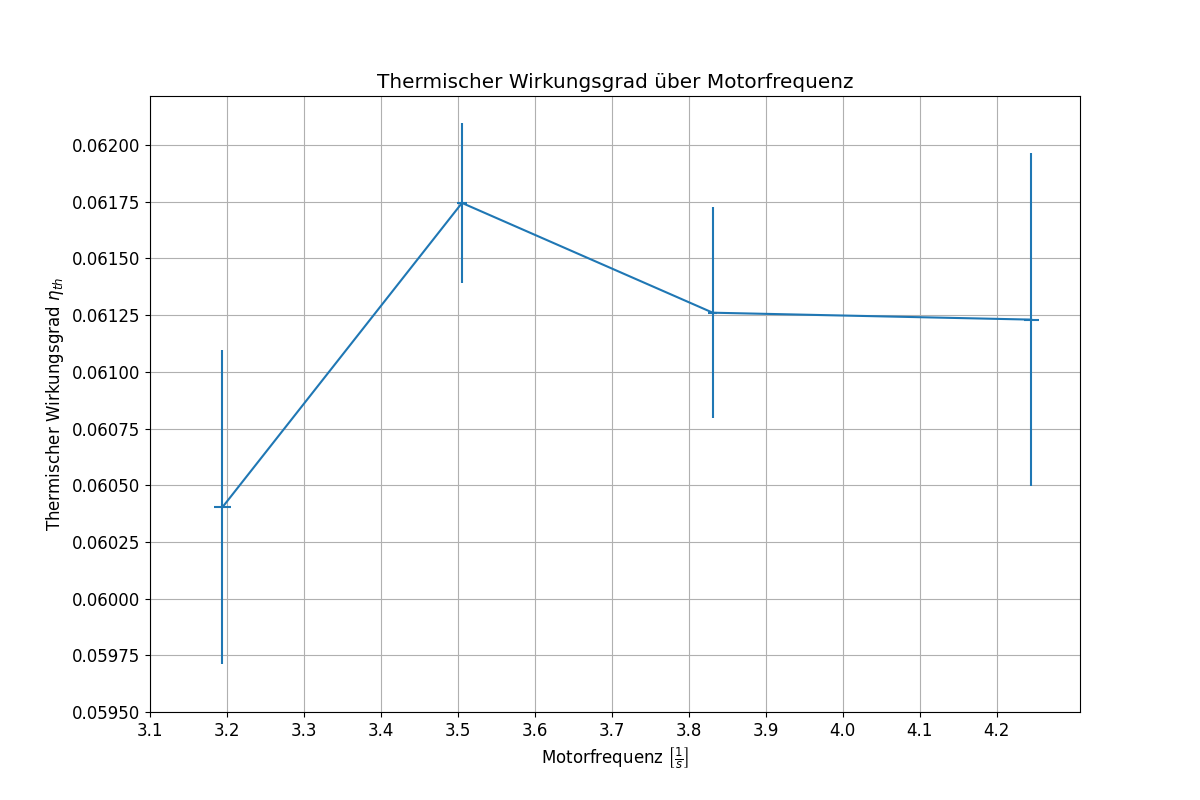
\includegraphics[width=.9\textwidth]{files/eta_th_freq.png}
    \caption{Thermischer Wirkungsgrad der Wärmekraftmaschine $\eta_{th}$ nach Motorfrequenz.}
    \label{fig:eta_th_freq}
\end{figure}


\begin{figure}[H]
    \centering
    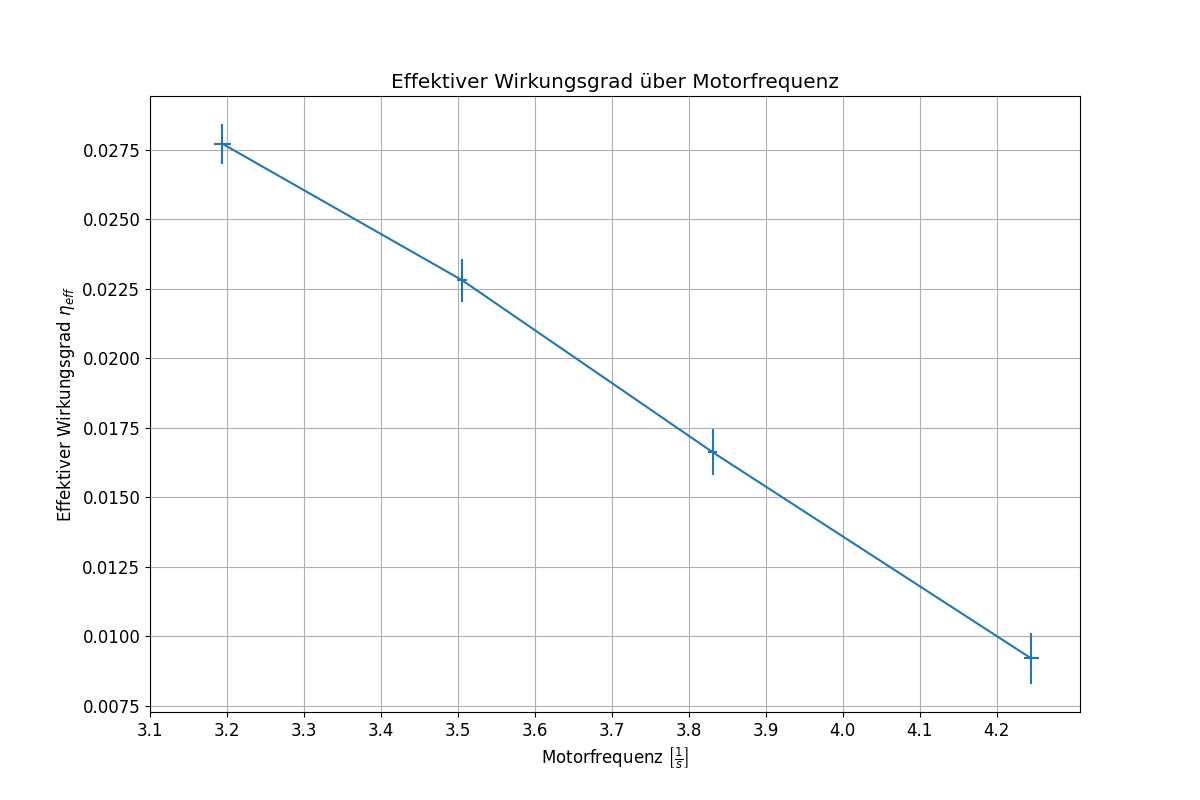
\includegraphics[width=.9\textwidth]{files/eta_eff_freq.png}
    \caption{Effektiver Wirkungsgrad der Wärmekraftmaschine $\eta_{th}$ nach Motorfrequenz.}
    \label{fig:eta_eff_freq}
\end{figure}